\documentclass[a4paper,10pt]{report}
% ---- graphiques
\usepackage[pdftex]{graphicx}
\usepackage{wrapfig}
\usepackage{color}
\usepackage{pst-tree}
%\usepackage{hyperref}

% for accents
\usepackage[latin1]{inputenc}
\usepackage[T1]{fontenc}

\usepackage{algorithm}
\usepackage{algorithmic}

\definecolor{darkgreen}{rgb}{0,0.4,0}
\definecolor{darkblue}{rgb}{0,0,0.4}
\definecolor{darkgray}{rgb}{0.2,0.2,0.2}

% ---- inclusion de codes
\usepackage{listings}
\lstset{showstringspaces=false,tabsize=4,basicstyle=\scriptsize\sffamily,breaklines=true,breakatwhitespace=true,framexleftmargin=5mm, frame=shadowbox, framesep=1pt,rulesepcolor=\color{darkgray},rulesep=.5pt,keywordstyle=\bf\color{blue},commentstyle=\color{magenta},stringstyle=\color{red},numbers=left,numberstyle=\tiny,numbersep=5pt,columns=flexible}

\lstdefinestyle{bash}{language=bash}
\lstdefinestyle{Perl}{language=Perl}
\lstdefinestyle{Python}{language=Python}
\lstdefinestyle{C++}{language=C++,emph={__global__,__shared__,__syncthreads,blockIdx,threadIdx,float3,float4},emphstyle=\bf\color{darkgreen}}
\lstdefinestyle{DTD}{language=XML}
\lstdefinestyle{XML}{language=XML,usekeywordsintag=false,markfirstintag=true}
%begin{latexonly}
\newcommand{\includecode}[2]{
\lstinputlisting[style=#1]{#2}
}
%end{latexonly}


%\lstnewenvironment{code}{}{}
\lstnewenvironment{code_bash}{\lstset{style=bash}}{}
\lstnewenvironment{code_perl}{\lstset{style=Perl}}{}
\lstnewenvironment{code_python}{\lstset{style=Python}}{}
\lstnewenvironment{code_cpp}{\lstset{style=C++}}{}
\lstnewenvironment{code_dtd}{\lstset{style=DTD}}{}
\lstnewenvironment{code_xml}{\lstset{style=XML}}{}

\newcommand{\textcode}[1]{{\sf #1}}




\newcommand{\sofa}{SOFA}
\newcommand{\todo}[1]{}
\newcommand{\eg}{\textit{e.g.} }

\renewcommand{\vec}[1]{\ensuremath{\mathbf{#1 }}} % vector
\newcommand{\Vx}{\vec{x} } % position vector
\newcommand{\Vv}{\vec{v} } % velocity vector
\newcommand{\Va}{\vec{a} } % acceleration vector
\newcommand{\Vf}{\vec{f}} % force
\newcommand{\Vdv}{\vec{\delta\Vv}} % change of velocity vector (unknown in implicit CG, and used in constraint solver
\renewcommand{\P}{\mat{P} } % projection to a constrained space.

\newcommand{\JNL}{\mathbf{\mathcal{J}} }     % mapping des positions
\newcommand{\J}{\mat J }                 % mapping lineaire
\newcommand{\M}{\mat M }             % matrice de masse
\newcommand{\K}{\mat K }             % matrice de raideur
\newcommand{\B}{\mat B }             % matrice d'amortissement
\newcommand{\G}{\mat G }             % jacobien des contraintes



% ---- inclusion de codes
\definecolor{darkgreen}{rgb}{0,0.4,0}
\definecolor{darkblue}{rgb}{0,0,0.4}
\definecolor{darkgray}{rgb}{0.2,0.2,0.2}


% macros mathematiques
\newcommand{\ma}[1]{\ensuremath{\mathbf {#1}}}
\newcommand{\ve}[1]{\ensuremath{\mathbf {#1}}}

\usepackage{amsmath}
\usepackage{amsfonts}
\usepackage{amssymb}

% character styles
\newcommand{\bm}[1]{\ensuremath{\mathbf{{#1}}}}
\newcommand{\mcal}[1]{\mbox{$\mathcal #1$}} % rondes math
\newcommand{\bmcal}[1]{\mbox{\boldmath $\mathcal #1$}} % rondes grasses math
\newcommand{\ensemble}[1]{\mbox{$\mathbb{#1}$}}
\newcommand{\RRR}{\mbox{$\ensemble{R}^3$}} 


% d�finitions
\newcommand{\definition}[2]{\index{#1}{\bf #1}: #2}
\newcommand{\voc}[1]{\index{#1}#1}
\newcommand{\bvoc}[1]{\index{#1}{\bf #1}}

% misc
\newcommand{\EV}[1]{\stackrel{\rightarrow}{#1}}  % espace vectoriel
\newcommand{\EA}[1]{#1}                          % espace affine

% vectors, matrices
%\newcommand{\point}[1]{\mbox{$#1$}}          % un point
\newcommand{\point}[1]{\ensuremath{#1}}          % un point
\newcommand{\mat}[1]{\bm{#1}}         % matrice
\newcommand{\matnm}[3]{\bm{#1_{#2\times #3}}}  % matrice n lignes , m colonnes
\newcommand{\vect}[1]{\bm{#1}}        % vecteur 
%\newcommand{\vecf}[1]{\stackrel{\rightarrow}{#1}}  % vecteur avec fleche
\newcommand{\vecf}[1]{\mbox{$\overrightarrow{#1}$}}  % vecteur avec fleche
\newcommand{\ident}[1]{\bm{I_{#1}}}   % identit� en dimension n
\newcommand{\inv}[1]{#1^{-1}}         % matrice inverse
\newcommand{\psinv}[1]{#1^{+}}        % matrice pseudo-inverse
\newcommand{\transp}[1]{#1^T}         % transpos�e de 1
\newcommand{\trace}[1]{tr(#1)}        % trace
\newcommand{\deter}[1]{\mbox{$|#1|$}}       % determinant
\newcommand{\oppvec}[1]{\mbox{$\left( \vect {#1} \wedge \right)$}}  % operateur matriciel de produit vectoriel

% bases, reperes
\newcommand{\vecin}[2]{\mbox{${}^{#2}#1$}}    % vecteur 1 dans repere 2
\newcommand{\Base}[1]{\ensuremath{\mathcal B_{#1}}} % Symbole du repere 1
\newcommand{\chbase}[3]{\mbox{${}_{#2}^{#3}\mat{#1}$}}  % operateur 1 fait le passage de la base 3 vers la base 2
%\newcommand{\pchbase}[2]{\chbase{\mat{B}}{#1}{#2}}  % matrice de passage de la base 2 vers la base 1
\newcommand{\pchbase}[2]{\chbase{B}{#1}{#2}}  % matrice de passage de la base 2 vers la base 1
\newcommand{\Rep}[1]{\ensuremath{\mathcal R_{#1}}} % Symbole du repere 1
\newcommand{\rep}[1]{\Rep{#1}}                 % Symbole du repere 1
%\newcommand{\pchrep}[2]{\chbase{\mat{F}}{#1}{#2}}  % matrice de passage du repere 1 vers le repere 2, F comme Frame
\newcommand{\pchrep}[2]{\chbase{\bm{C}}{#1}{#2}}  % matrice de passage du repere 2 vers le repere 1

%% Operateur de passage du repere 1 par rapport a 2
%\newcommand{\ChgRep}[2]{\mbox{\boldmath $R_{#1}^{#2}$}}

% rotations	
%\newcommand{\rot}[2]{\mbox{$\mat{R}_{#1,#2}$}}      % rotation vectorielle
\newcommand{\rot}[2]{\ensuremath{\mat{R}_{#1,#2}}}      % rotation vectorielle
\newcommand{\rota}[3]{\mbox{$\mat{R}_{#1,#2,#3}$}}  % rotation affine

% translation
\newcommand{\trans}[2]{\mbox{$\chbase{\vect{t}}{#1}{#2}$}} % passage de #1 vers #2 par une translation, ou translation du repere #2 par rapport au repere #1

% vitesses et acc�l�rations
\newcommand{\VRep}[2]{\mbox{\boldmath $\dot R_{#1}^{#2}$}} % vitesse du repere 1 par rapport a 2 
%\newcommand{\Point}[2]{\mbox{\boldmath ${#1}^{#2}$}}  % Coordonnees d'un point 1 dans un repere 2
\newcommand{\Point}[2]{\mbox{$\vecin{\bm{#1}}{#2}$}}  % Coordonnees d'un point 1 dans un repere 2
\newcommand{\VPoint}[2]{\mbox{\boldmath ${\dot #1}_{/#2}$}} % Vitesse d'un point par rapport � un repere
\newcommand{\APoint}[2]{\mbox{\boldmath ${\ddot #1}_{/#2}$}} % Acceleration d'un point par rapport � un repere

% cinematique du solide
\newcommand{\derivedans}[2]{\mbox{$\dot{#1}^{(#2)}$}}  % derivee du vecteur 1 dans repere 2
\newcommand{\fixedans}[2]{\mbox{$#1_{\in #2}$}}        % vecteur 1 fixe dans repere 2
\newcommand{\vecom}{\mbox{$\bm{\Omega}$}}  % omega de 1 par rapport a 2
\newcommand{\vecrot}[2]{\mbox{$\vecom_{#1/#2}$}}  % omega de 1 par rapport a 2
\newcommand{\accrot}[2]{\mbox{$\dot{\vecom}_{#1/#2}$}}  % omega de 1 par rapport a 2
\newcommand{\vfdans}[3]{\mbox{$\vec V^{#2/#3}_{#1}$}}    % vitesse de 1 fixe dans 2 par rapport a 3
\newcommand{\afdans}[3]{\mbox{$\vec \Gamma^{#2/#3}_{#1}$}}    % acceleration de 1 fixe dans 2 par rapport a 3
\newcommand{\vmdans}[2]{\mbox{$\vec V^{/{#2}}_{#1}$}}    % vitesse de 1 mobile dans 2
\newcommand{\amdans}[2]{\mbox{$\vec \Gamma^{/#2}_{#1}$}}    % acceleration de 1 mobile dans 2

% chaines articulees
\newcommand{\liaison}[2]{\mbox{$\mathcal L_{#1,#2}$}}  % liaison du pere 1 vers fils 2 (et repere intermediaire)
\newcommand{\liaisonprime}[2]{\mbox{$\mathcal L'_{#1,#2}$}}  % deuxieme repere intermediaire de la liaison du pere 1 vers fils 2
\newcommand{\liaisonP}[2]{\mbox{$\mathcal L_{#1,#2}$}}  % Repere dans pere 1 de la liaison vers fils 2 
\newcommand{\liaisonC}[2]{\mbox{$\mathcal L'_{#1,#2}$}}  % Repere dans fils de la liaison du pere 1 vers fils 2 
%\newcommand{\transP}[2]{\pchrep{\liaisonP{#1}{#2}}{#1}}  % Matrice du repere dans pere de la liaison du pere 1 vers fils 2 
%\newcommand{\transC}[2]{\pchrep{\liaisonC{#1}{#2}}{#2}}  % Matrice du repere dans pere de la liaison du pere 1 vers fils 2 
%\newcommand{\transPC}[2]{\pchrep{\liaisonC{#1}{#2}}{\liaisonP{#1}{#2}}}  % matrice de passage entre repere liaison dans fils et repere de liaison dans pere
\newcommand{\transP}[2]{\chbase{C_p}{#2}{#1}}  % Matrice du repere dans pere de la liaison du pere 1 vers fils 2 
\newcommand{\transC}[2]{\chbase{C_c}{#2}{#1}}  % Matrice du repere dans pere de la liaison du pere 1 vers fils 2 
\newcommand{\transPC}[2]{\chbase{C_l}{#2}{#1}}  % matrice de passage entre repere liaison dans fils et repere de liaison dans pere
% \pchrep{fils}{pere} = \liaisonP{pere}{fils}\deplPC{pere}{fils}\liaisonC{pere}{fils}


\newcommand{\pctab  }{\hspace{0.15in}      }  % Pseudo-code indentation.
\newcommand{\code}[1]{ 
\begin{makeimage}
\begin{tabbing} \pctab \= \pctab \= \pctab \= \pctab \= \pctab \= \pctab \= \pctab \kill
#1
\end{tabbing}
\end{makeimage}
}
 % Customizations 

% ---- format de page A4
	\setlength{\textwidth }{16cm}	% largeur de ligne
	\setlength{\textheight}{23cm}   % hauteur du texte
	\setlength{\oddsidemargin}{0cm} % marge pages impaires
	\setlength{\evensidemargin}{0cm}% marge pages paires
	\setlength{\topmargin}{0cm} 	

% Title Page
\title{Sofa Documentation}
\author{The Sofa Team}



\begin{document}
\maketitle

\begin{abstract}
This is the Sofa documentation
\end{abstract}

\tableofcontents

% This chapter is borrowed from a stand-alone document defined in directory introduction/
\chapter{Introduction to \sofa}
\graphicspath{{introduction/}}  % to include images

\section{Why \sofa ?}
% The creation of geometric models can require complex algorithms for surface extraction, mesh simplification or refinement and volumetric meshing.
Programming interactive physical simulation of rigid and deformable objects requires multiple skills in geometric modeling, computation mechanics, numerical analysis, collision detection, rendering, user interface and haptics feedback, among others. 
It is also challenging from a software engineering standpoint, with the need for computationally efficient algorithms, multi-threading, or the deployment of applications on modern hardware architectures such as the GPU.
The development of complex medical simulations has thus become an increasingly complex task, involving more domains of expertise than a typical research and development team can provide.
The goal of \sofa{} is to address these issues within a highly modular yet efficient framework, to allow researchers and developers to focus on their own domain of expertise, while re-using other expert's contributions. 

\section{The "philosophy" of \sofa}
\sofa{} introduces the concept of multi-model representation to easily build simulations composed of complex anatomical structures.
The pool of simulated objects and algorithms used in a simulation (also called a scene) is described using a hierarchical data structure similar to scene graphs used in graphics libraries. 
Simulated objects are decomposed into collections of independent components, each of them describing one feature of the model, such as state vectors, mass, forces, constraints, topology, integration scheme, and solving process.
As a result, switching from internal forces based on springs to a finite element approach can be done by simply replacing one component with another, all the rest (mass, collision models, time integration, ...) remaining unchanged. Similarly, it is possible to keep the same force model and modify the solver and state vectors in order to compute the model on the GPU instead of the CPU.
 Moreover, the simulation algorithms, embedded in components, can be customized with the same flexibility as the physical models.

In addition to this first level of modularity, it is possible to go one step further and decompose simulated objects into multiple partial models, each optimized for a given type of computation.
Typically, a physical object in \sofa{} is described using three partial models: a mechanical model with mass and constitutive laws, a collision model with contact geometry, and a visual model with detailed geometry and rendering parameters.
Each model can be designed independently of the others, and more complex combinations are possible, for instance for coupling two different physical objects.
During run-time, the models are synchronized using a generic mechanism called \textit{mapping} to propagate forces and displacements. 
The user can interact in real-time with the mechanical models simulated in SOFA, using the mouse but also using other type of input device. Haptic rendering is also supported.
% \SC{This mapping can simply update the position of vertices on the visual model, or transmit forces and velocities between the collision model and mechanical model. In this case the mapping follows the physical principle of the \textit{virtual works}.} \ff{(Mapping trop détaillé ici à mon avis)}

\section{Why should I contribute to \sofa ?}
\sofa{} was first released in 2007~\cite{ACFBPDDG07}. Since then, it has evolved toward a comprehensive, high-performance library used by an increasing number of academics and commercial companies.
The code is open-source and the license is LGPL. 
 You can use this code to build your own medical simulations needs or for other applications. You can also include this code in a commercial product. 
The only requirement is that if you modify the code for a commercial product you need to share this modification with your client.

Moreover, you can build upon SOFA using the plug-in system. Your plug-in can have an other license than LGPL. Consequently there is a considerable freedom for you to use SOFA for your research, your developments or your products !

Finally,  \sofa is also intended for the research community to help the development and the sharing of newer algorithms and models.
So, do not hesitate to share your experience of \sofa, your code and your results with the \sofa community !!!



% This chapter is borrowed from a stand-alone document defined in directory design/
\chapter{Design}
\graphicspath{{design/}}  % to include images
\begin{wrapfigure}{r}{0.5\textwidth}%
\centering%
\vspace{-1cm}
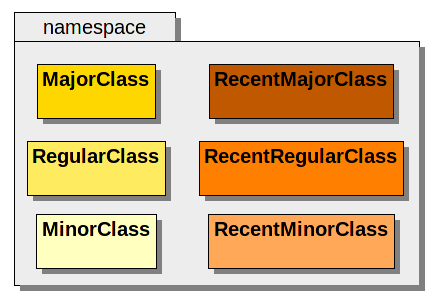
\includegraphics[scale=.33]{../classdiagrams/uml-legend.png}%
\caption{Color conventions in UML diagrams.}%
\label{fig:uml-legend}%
\end{wrapfigure}%

\section{Introduction}

This chapter present the design of \sofa{}, as well as its recent evolutions.
It also includes discussions justifying some of the decision that are behind this design.

The conventions used in UML class diagrams are presented in Fig~\ref{fig:uml-legend}.

\vspace{.8cm}

\section{Core Class Diagrams}

\subsection{Object Model (\textcode{sofa::core::objectmodel})}

\begin{figure}[h]
\centering
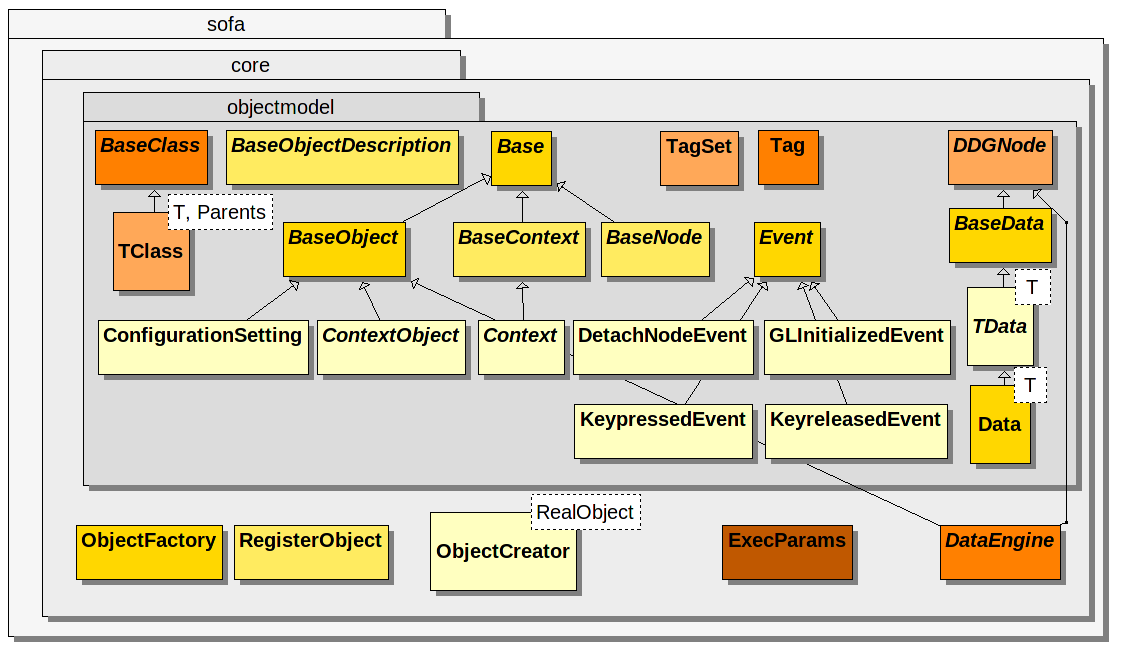
\includegraphics[scale=.33]{../classdiagrams/sofacore-objectmodel.png}
\caption{Classes of the \textcode{sofa::core::objectmodel} namespace.}
\label{fig:uml-sofa-core-objectmodel}
\end{figure}

\subsubsection{Changes compared to the 1.0~beta~4 version}\label{sec:design-core-objectmodel-changes}

\paragraph{New class description system.}
It is based on the \textcode{BaseClass} and \textcode{TClass} classes, and requires to add the \textcode{SOFA\_CLASS} macro in the declaration of all classes deriving from Base.
The benefits are that it is now possible to follow the full hierarchy of classes from the final components, instead of having just a fixed set of categories.
This macro is also necessary in classes with a templated parent class to be able to use methods and member variables defined in \textcode{Base} such as \textcode{initData} or \textcode{sout}. This removed all the previously redundant direct heritage to \textcode{BaseObject} that was previously required.

\paragraph{Objects and node tagging (\textcode{Tag} and \textcode{TagSet}).}
The goal of the introduction of tags is to provide one of the pieces necessary to support non-mechanical states (electrical potentials, constrast agent concentrations) as well as cleaner non-geometrical mechanical states (fluid dynamics, reduced-coordinate articulations).
For example, in a simulation involving blood in deformable vessels, we would use two tags to distinguish the different states : mechanical, fluid.
These tags will be used to easily work with only a subset of the components, so that the mechanical solver works on positions and forcefields but don't interferes with blood flow and pressure, and inversely for the fluid solver\footnote{\url{http://wiki.sofa-framework.org/tdev/wiki/Notes/ProposalGenericStates}}.
We decided on using there tags instead of extending the class hierarchy as was done before with the \textcode{State} and \textcode{MechanicalState} classes.
A hierarchy is fine when we have only one feature that we want to differentiate on (such as base vs mechanical vs electrical), but when we add other criteria (lagrangian geometry vs eulerian vs reduced generalized coordinates, velocity vs vorticity, independent vs mapped DOFs) it is no longer manageable as specialized classes.
A secondary use of these tags is to replace existing subsets mechanisms within CollisionModels (r2441) and Constraints (r3121).
The design is based on the following elements.
Tags are added to BaseObject, as a list of string (internally converted to a list of unique ids for faster processing).
All visitors now filter the objects they process based on their list of tags.
All solvers by default copy their own list of tags to the visitors they execute, so that they only affect the objects with the same tags as they have (TODO: this is currently broken). 

\paragraph{Dependencies between Data (\textcode{DDGNode} and \textcode{DataEngine}).}
The goal is to be able to specify simple links between datas or through computation engines.
To function correctly, the methods \textcode{getValue()} or \textcode{beginEdit()}/\textcode{endEdit()} are required to be called in all codes accessing values contained in Data instances.
To enforce this, the class DataPtr was removed.
Note also that it is very inefficient to call \textcode{getValue()} repetively within computation loops.
Instead, the recommanded method is to use the helper classes \textcode{ReadAccessor} and \textcode{WriteAccessor}
that can hold a reference to a \textcode{Data} value, provides the same API as regular vectors,
and automatically calls \textcode{endEdit()} at the end of the call block in case of \textcode{WriteAccessor}.

\textbf{TODO:} \textit{\textcode{TData<T>} was useful as a common parent for \textcode{Data<T>} and \textcode{DataPtr<T>}, but now that \textcode{DataPtr} no longer exist, it would simplify the hierarchy to merge \textcode{TData<T>} and \textcode{Data<T>}.}

\paragraph{\textit{Copy-on-Write} (CoW) mechanism (\textcode{DataContainer}).}
The goal is to reduce copies of datas when using engines and/or multi-threading.
It is completly transparent to other codes, since everything should now respect the data access API (see above).
There is however one important side-effect that may break some existing code: the pointer to the value of a \textcode{Data} can now change during a call to \textcode{beginEdit()}.
This means that it is now illegal to retrieve the pointer to the value in a \textcode{Data} at init time and then reuse it after edits might have been made.

\paragraph{Support for asynchronous multi-threading (\textcode{ExecParams}).}
This feature is an important goal of the new design, however it is not yet completely functionnal and thus may change shortly.


\subsection{Physical Behavior (\textcode{sofa::core::behavior})}
\begin{figure}[h]
\centering
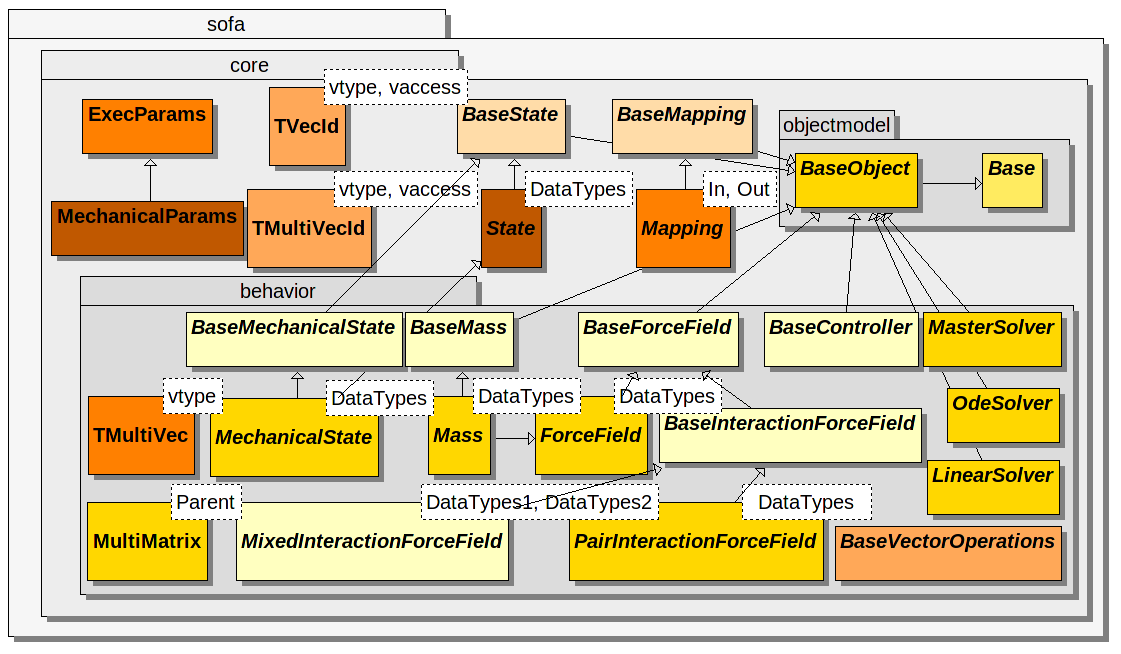
\includegraphics[scale=.33]{../classdiagrams/sofacore-behavior.png}
\caption{Classes of the \textcode{sofa::core::behavior} namespace.}
\label{fig:uml-sofa-core-behavior}
\end{figure}

\subsubsection{Changes compared to the 1.0~beta~4 version}\label{sec:design-core-behavior-changes}

\paragraph{\textcode{VecId} is replaced by templated classes to specify vector types and read/write access.}

Previously, the \textcode{VecId} class was used by solvers and visitors to specify on which state vectors should an operation be applied.
However, this API did not express the requirements for these vectors (which type, i.e. \textcode{Coord}, \textcode{Deriv}, or \textcode{MatDeriv}), nor if they were supposed to be read or written.
Now, methods and visitors can use the following classes instead (all typedefs from a common \textcode{TVecId} templated class), so that developers will now explicitly what to expect:

\begin{code_cpp}
/// Identify one vector stored in State
/// A ConstVecId only provides a read-only access to the underlying vector.
typedef TVecId<V_ALL, V_READ> ConstVecId;

/// Identify one vector stored in State
/// A VecId provides a read-write access to the underlying vector.
typedef TVecId<V_ALL, V_WRITE> VecId;

/// Typedefs for each type of state vectors
typedef TVecId<V_COORD, V_READ> ConstVecCoordId;
typedef TVecId<V_COORD, V_WRITE>     VecCoordId;
typedef TVecId<V_DERIV, V_READ> ConstVecDerivId;
typedef TVecId<V_DERIV, V_WRITE>     VecDerivId;
typedef TVecId<V_MATDERIV, V_READ> ConstMatrixDerivId;
typedef TVecId<V_MATDERIV, V_WRITE>     MatrixDerivId;
\end{code_cpp}

Also, a new class \textcode{TMultiVecId} is introduced to be able to specify different IDs for specific states or groups of states. Similar typedefs are defined as above, replacing \textcode{Vec} with \textcode{MultiVec}.

\paragraph{New State API and class hierarchy.}
The previous State API was based on \textcode{getX()}/\textcode{getV()}/... methods that returned pointers to the vectors last specified (using \textcode{setX()}/\textcode{setV()}/... methods) as the current position, velocity, ...
This is now replaced by \textcode{read(ConstVec\textit{TYPE}Id)} and \textcode{write(Vec\textit{TYPE}Id)} methods, where \textcode{\textit{TYPE}} is either \textcode{Coord}, \textcode{Deriv}, or \textcode{MatDeriv}.
These methods return a pointer to a Data instance containing the vector, instead of the vector itself.
This was necessary to respect the Data access API (see section~\ref{sec:design-core-objectmodel-changes}).
For compatibility with existing codes (especially \textcode{draw()} methods), the read-only \textcode{getX()}/\textcode{getV()}/... methods still exists but they are deprecated (and there are strictly equivalent to calling \textcode{read()} with the default ID for position, velocity, ...).
The non-const versions however are removed, so all codes modifying state vectors will have to use the new Data-based API.
Note that with this change, the state components no longer store the information about which vectors should be considered as the current position, velocity, ...
So another mechanism is required to specify these associations (\textcode{MechanicalParams}, see below).

A new state class hierarchy is also defined,  introducing a new parent class \textcode{BaseState}, common to all states (mechanical, visual, ...).
Methods allowing to read and write vectors given their IDs are specified in \textcode{State<DataTypes>}.
The \textcode{MappedModel} class is removed, non-mechanical state components (such as visual models) now directly derive from \textcode{State<DataTypes>}.


\paragraph{Simplified \textcode{Mapping} class hierarchy.}
Previously, a different base class (\textcode{Mapping< State<TIn>, MappedModel<TOut> >} or \textcode{MechanicalMapping< MechanicalState<TIn>, MechanicalState<TOut> >}) where used for mechanical versus non-mechanical (i.e. visual or one-way) mappings.
This introduced complexities and redundancies in the code of the final components (they where templated by the type of their parent class and compiled twice for each pair of input/output datatypes).
Now, a single base class is used (\textcode{Mapping<TIn,TOut>}, templated only by the input and output datatypes.
Components are also templated by the same types, similarly to other classes such as forcefields.
A new set of flags is used to check if a given mapping is mechanical or not.
Different flags are used to activate the mapping of forces, masses, and constraints separatly (although by default they have the same value).
Components that do not implement applyJT (i.e. visual mappings) can force them to false to indicate they do not support mechanical computations.

\paragraph{New mechanical component API based on \textcode{Data} and \textcode{MechanicalParams}.}
This is the most important change from the previous design.
To provide all the required vector IDs that where previously stored within each \textcode{MechanicalState} by calls to \textcode{setX()}/... methods, we define a \textcode{MechanicalParam} class.
This class is given to all mechanical-related methods, specified by \textcode{OdeSolver}s and transmitted by \textcode{MechanicalVisitor}s.
It hides the \textcode{VecId} system from most component codes, providing the same abstraction of accessing the current position and velocity vectors as was previously handled within \textcode{MechanicalState}. For example, where a component such as a \textcode{ForceField} implementation used :
\begin{code_cpp}
const VecCoord* x = this->mstate->getX();
\end{code_cpp}
It will now use \textcode{MechanicalParams} as follows :
\begin{code_cpp}
helper::ReadAccessor<VecCoord> x = *mparams->readX(this->mstate);
\end{code_cpp}

This API is preferable to directly manipulating \textcode{VecId}s (such as in \textcode{this->mstate->read(mparams->getXId(this->mstate))}) because :
\begin{itemize}
\item The code is very similar to the previous version.
\item If the API of the \textcode{VecId} or \textcode{MechanicalState} class is further changed, the \textcode{MechanicalParam::readX()} method can handle it.
\item Different \textcode{VecId}s for different states can be chosen within \textcode{MechanicalParam} (such as what is currently used for free vs mapped states, and animated vs external obstacle state).
\end{itemize}

However it is still possible to get the ids (using \textcode{mparams->x().getId(mstate)}).

All vector accesses given though \textcode{MechanicalParams} are read-only.
Vectors actually modified by each method are given as separate \textcode{MultiVecId} parameters.
This is useful to make the API clearer (we can see explicitly what each method is supposed to write) and safer (no accidental modifications to X or V within \textcode{addForce()} or \textcode{draw()} for example).
Finally, other interesting pieces of information can be queried though \textcode{MechanicalParams}.
For example, a ForceField can know as soon as the \textcode{addForce()} call if the current solver is implicit or explicit, if the kinematic and potential energy should be computed, ...

\paragraph{New solver hierarchy and vector manipulation API (\textcode{TMultiVec} and \textcode{BaseVectorOperations}).}
Previously, the solver classes had a complex hierarchy, with several parent classes (\textcode{SolverImpl}, \textcode{OdeSolverImpl}, \textcode{MasterSolverImpl}) that where used to launch each type of visitors (mechanics, linear algebra, ...).
In the new design, these classes are replaced by separate helper classes (\textcode{VectorOperations}, \textcode{MechanicalOperations}) that are instanciated at runtime and allow to launch each type of visitors while holding and updating the persistant parameters (in the form of a \textcode{MechanicalParams} for mechanical visitors for example, or \textcode{ExecParams} for simple vector operations).


\subsection{Topology (\textcode{sofa::core::topology})}

\textit{The design of this namespace is still a work in progress, so major changes should still be expected...}

\subsubsection{Changes compared to the 1.0~beta~4 version}

\textit{To be documented...}

\subsection{Collision (\textcode{sofa::core::collision})}

\begin{figure}[h]
\centering
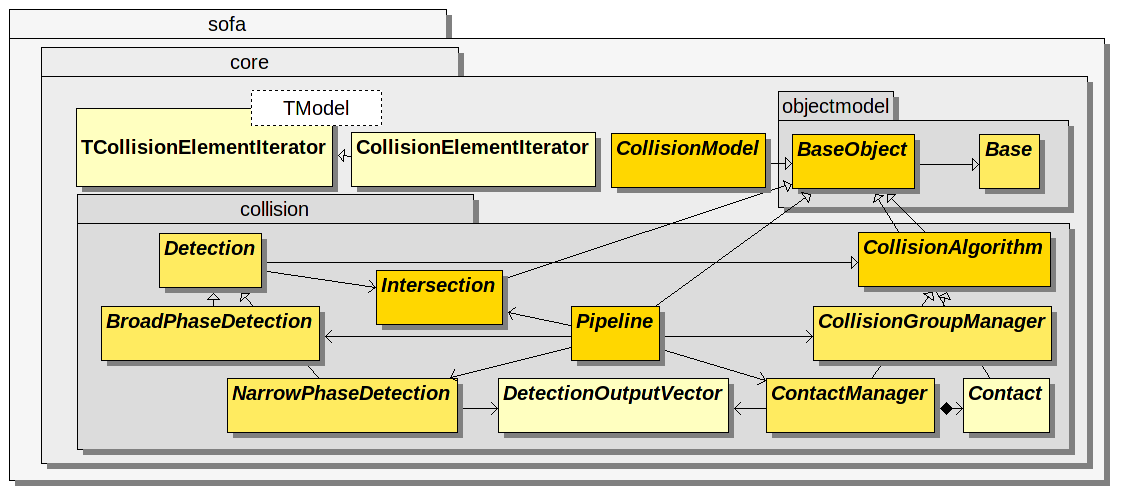
\includegraphics[scale=.33]{../classdiagrams/sofacore-collision.png}
\caption{Classes of the \textcode{sofa::core::collision} namespace.}
\label{fig:uml-sofa-core-collision}
\end{figure}

\subsubsection{Changes compared to the 1.0~beta~4 version}

\textit{No major changes.}

\subsection{Mesh and Image Loaders (\textcode{sofa::core::loader})}

\begin{figure}[h]
\centering
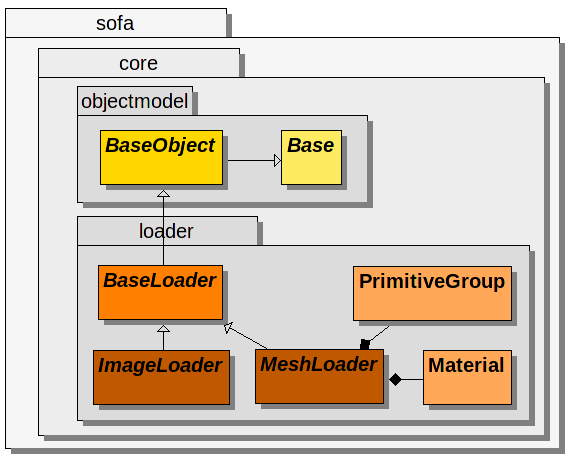
\includegraphics[scale=.33]{../classdiagrams/sofacore-loader.png}
\caption{Classes of the \textcode{sofa::core::loader} namespace.}
\label{fig:uml-sofa-core-loader}
\end{figure}

\subsubsection{Changes compared to the 1.0~beta~4 version}

This namespace is completely new.

\textit{To be documented...}

\pagebreak

\section{Main classes}

\subsection{\textcode{sofa::core::objectmodel}}

\subsubsection{\textcode{Base}}

\lstinputlisting[style=C++,linerange=51-181]{../../framework/sofa/core/objectmodel/Base.h}

\subsubsection{\textcode{BaseObject}}

\lstinputlisting[style=C++,linerange=61-160]{../../framework/sofa/core/objectmodel/BaseObject.h}

\subsection{\textcode{sofa::core}}

\subsubsection{\textcode{BaseState}}

\lstinputlisting[style=C++,linerange=39-58]{../../framework/sofa/core/BaseState.h}

\subsubsection{\textcode{State}}

\lstinputlisting[style=C++,linerange=38-103]{../../framework/sofa/core/State.h}

\subsubsection{\textcode{BaseMapping}}

\lstinputlisting[style=C++,linerange=48-116]{../../framework/sofa/core/BaseMapping.h}

\subsubsection{\textcode{Mapping}}

\lstinputlisting[style=C++,linerange=43-115]{../../framework/sofa/core/Mapping.h}


%% \section{Framework}

%% \subsection{UML Diagrams}

%% \begin{figure}[h]
%% \centering
%% 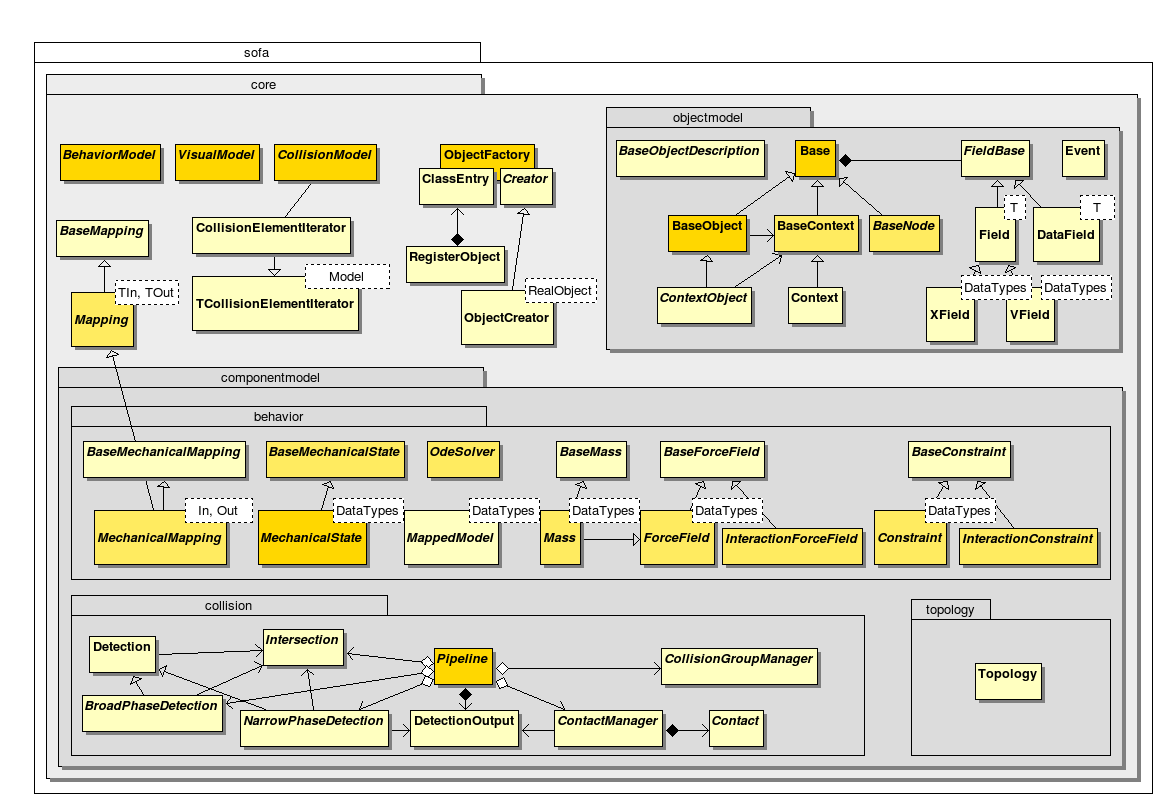
\includegraphics[width=\linewidth]{uml-sofa-core.png}
%% \caption{Classes of the sofa::core namespace.}
%% \label{fig:uml-sofa-core}
%% \end{figure}


% This chapter is defined here
\chapter{How to contribute to this documentation}
\section{Document structure}
This document gathers the content of other documents located in different subdirectories. These documents can also be compiled as stand-alone documents.
The structure can be illustrated as follows:
\begin{itemize}
 \item \texttt{sofadocumentation.tex} : the root document.
 \item \texttt{macros\_docu.tex} : custom commands and macros. This file is included by the root document.
 \item \texttt{introduction} : a subdirectory containing a chapter of this document.
\begin{itemize}
 \item \texttt{introduction.tex} : a stand-alone article containing the same. This file may include \texttt{../macros\_docu.tex} to use the common custom commands.
 \item \texttt{introduction\_body.tex} : the text of the chapter/article. This file is included as a chapter by \texttt{sofadocumentation.tex}, and included as full article text by \texttt{introduction.tex}.
\end{itemize}
 \item there could (and hopefully will !) be other subdirectories with a similar structure.
\end{itemize}

\section{Compiling the document}
\subsection{File formats}
The graphics are handled by: \texttt{\textbackslash usepackage[pdftex]\{graphicx\}}. This allows the inclusion of \texttt{.png} images rather than \texttt{.eps}, which makes the image files much smaller, and compilation of \texttt{html} faster. The result of the compilation is a \texttt{.pdf} rather than a \texttt{.dvi} file.

\subsection{Include paths}
The root document includes files in the subdirectories, which in turn include files too. The problem is that the path from the subdirectory (used when compiling a stand-alone article) is not the same as from the parent directory (used when compiling the whole report).
It seems that \LaTeX has no include path command to circumvent this problem.

Fortunately, \LaTeX uses an environment variable named TEXINPUTS which represents a list of directories to search. We use this variable to allow file inclusion, by adding the parent directories to the list. The command lines depend on the shell, e.g.:
\begin{itemize}
 \item using bash: \texttt{export TEXINPUTS=\$\{TEXINPUTS\}:..:../.. ; latex sofadocumentation.tex}
 \item using tcsh: \texttt{setenv TEXINPUTS \$\{TEXINPUTS\}:..:../.. ; latex sofadocumentation.tex}
\end{itemize}

Using the \texttt{Kile} graphical front-end, you can customize the command line in menu \texttt{Settings/Kile/Tools/Build}, select tool \texttt{LATEX} and write the appropriate command line in the \texttt{Command} field.

\subsection{HTML}
HTML can be generated using the following command:\\
\texttt{latex2html sofadocumentation.tex -mkdir -dir ./html -show\_section\_numbers -split 1}
\\
Currently, the listings do not appear in html.

\end{document}          
